	\paragraph{QuizziPedia::Front-End::ModelViews::ProfileManagementModelView}
	
	\label{QuizziPedia::Front-End::ModelViews::ProfileManagementModelView}
	
	\begin{figure}[ht]
		\centering
		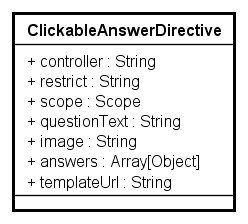
\includegraphics[scale=0.5,keepaspectratio]{UML/Classi/Front-End/QuizziPedia_Front-end_Templates_ClickableAnswerTemplate.png}
		\caption{QuizziPedia::Front-End::ModelViews::ProfileManagementModelView}
	\end{figure} \FloatBarrier
	
	\begin{itemize}
		\item \textbf{Descrizione}: classe di tipo modelview la cui istanziazione è contenuta all'interno della variabile di ambiente \$scope di \textit{Angular.js\ped{G}}. All'interno di essa sono presenti le variabili e i metodi necessari per il \textit{Two-Way Data-Binding\ped{G}} tra la view \texttt{ProfileManagementView} e il controller \texttt{ProfileManagementController};
		\item \textbf{Utilizzo}: viene utilizzata per effettuare il \textit{Two-Way Data-Binding\ped{G}} tra la view \texttt{ProfileManagementView} e il controller \texttt{ProfileManagementController} rendendo disponibili variabili e metodi;
		\item \textbf{Relazioni con altre classi}: 
		\begin{itemize}
			\item \textit{IN} \texttt{ProfileManagementView}: view contenente i dati personali che un utente può modificare dopo essersi registrato al sistema; 
			\item \textit{IN} \texttt{ProfileManagementController}: questa classe permette di gestire il profilo personale di un utente;
		\end{itemize}
		\item \textbf{Attributi}: 
		\begin{itemize}
				\item \texttt{+ name} \\ Campo dati che conterrà il nome dell'utente;
				\item \texttt{+ surname} \\ Campo dati che conterrà il cognome dell'utente;
				\item \texttt{+ email} \\ Campo dati che conterrà l'email dell'utente;
				\item \texttt{+ image} \\ Campo dati che conterrà l'immagine del profilo dell'utente;
				\item \texttt{+ password} \\ Campo dati che conterrà la password dell'utente;
				\item \texttt{+ passwordCheck} \\ Campo dati che conterrà la password di conferma dell'utente.
		\end{itemize}
		\item \textbf{Metodi}: 
		\begin{itemize}
			\item \texttt{+} \texttt{confirm(): void} \\
			Metodo che gestisce l’evento click sul pulsante di conferma modifica. Aggiorna, in caso di modifiche, l'oggetto locale \texttt{UserDetailsModel}. Inoltre, utilizzando il metodo dell'\texttt{UserDetailsService}, aggiorna anche nel server i dati dell'utente.
		\end{itemize}
	\end{itemize}	

